\chapter{三维场景技术基础}

\paragraph*{学习目标}

通过本章学习，学生应能够：

\begin{enumerate}
\def\labelenumi{\arabic{enumi}.}
\tightlist
\item
  \textbf{掌握三维场景核心概念}：理解三维场景技术在智慧水利中的基础作用，掌握三维图形学基本原理
\item
  \textbf{熟练掌握WebGL与Three.js}：熟悉WebGL技术架构，掌握Three.js开发框架的核心API和使用方法
\item
  \textbf{掌握三维建模技术}：掌握几何建模、纹理贴图、材质系统等建模技术的基本方法
\item
  \textbf{理解基础渲染技术}：了解光照模型、阴影渲染、材质系统等基础图形渲染技术
\item
  \textbf{具备基础开发能力}：能够使用主流三维开发框架构建简单的水利场景应用
\item
  \textbf{建立技术认知体系}：为后续章节的学习提供必要的技术基础
\end{enumerate}

\paragraph*{引言}

三维场景技术是智慧水利平台的重要基础，为水利工程信息提供直观的可视化表达。本章按照 ``WebGL 与 Three.js 三维渲染基础 - GIS 地图服务集成 - BIM 与倾斜摄影模型构建 - 数字孪生架构'' 的逻辑展开，既介绍浏览器端三维渲染的基本原理，也说明智慧水利场景中地图、工程模型、实景模型和实时监测数据如何逐步融合，最终支撑数字孪生平台建设。

\section{WebGL与Three.js三维渲染基础}

\subsection{三维图形学基础概念}

三维渲染的核心是将虚拟三维世界的信息经过一系列变换和计算，最终投影到二维屏幕上显示给用户。这个过程涉及多个坐标系统和变换矩阵，是理解WebGL和Three.js的必要基础。

\textbf{坐标系统与齐次坐标}

三维图形学中常用三种主要坐标系统：
\begin{itemize}
\item \textbf{局部坐标系（Local Coordinate）}：模型相对于自身中心的坐标系，通常由建模软件或几何定义直接提供。例如一个水闸模型，其坐标原点通常在模型的中心或基底。
\item \textbf{世界坐标系（World Coordinate）}：整个三维场景的全局坐标系，所有模型最终都需要变换到世界坐标系中。对于水库场景，世界坐标系通常以工程基准点或地理坐标转换后的点作为原点。
\item \textbf{屏幕坐标系（Screen/Viewport Coordinate）}：二维屏幕坐标，左上角通常为 $(0, 0)$，右下角为 $(width, height)$。深度信息存储在Z缓冲区中。
\end{itemize}

在计算机图形学中，为了统一表示平移、旋转和缩放等所有仿射变换，采用\textbf{齐次坐标}表示三维点。三维笛卡尔坐标 $(x, y, z)$ 对应齐次坐标 $(x, y, z, 1)$；方向向量则表示为 $(dx, dy, dz, 0)$（注意最后一个分量为0）。这样做的优势是所有变换都可以用矩阵乘法统一表示。

\textbf{基本变换矩阵}

三维仿射变换包括平移、旋转和缩放，分别对应以下矩阵：

平移变换（沿向量 $\mathbf{t} = (t_x, t_y, t_z)$）：
$$T(\mathbf{t}) = \begin{pmatrix} 1 & 0 & 0 & t_x \\ 0 & 1 & 0 & t_y \\ 0 & 0 & 1 & t_z \\ 0 & 0 & 0 & 1 \end{pmatrix}$$

缩放变换（缩放因子 $(s_x, s_y, s_z)$）：
$$S(s_x, s_y, s_z) = \begin{pmatrix} s_x & 0 & 0 & 0 \\ 0 & s_y & 0 & 0 \\ 0 & 0 & s_z & 0 \\ 0 & 0 & 0 & 1 \end{pmatrix}$$

旋转变换围绕Z轴旋转角度 $\theta$：
$$R_z(\theta) = \begin{pmatrix} \cos\theta & -\sin\theta & 0 & 0 \\ \sin\theta & \cos\theta & 0 & 0 \\ 0 & 0 & 1 & 0 \\ 0 & 0 & 0 & 1 \end{pmatrix}$$

在实际应用中，模型变换（Model Matrix）将顶点从局部坐标变换到世界坐标；视图变换（View Matrix）将世界坐标变换到相机坐标系；投影变换（Projection Matrix）将相机坐标投影到齐次裁剪坐标。这些变换的组合称为\textbf{模视投矩阵}（Model-View-Projection Matrix，MVP矩阵）。

\textbf{投影变换}

投影是将三维场景投影到二维平面的关键步骤，分为正交投影和透视投影两类。

正交投影（Orthographic Projection）不考虑距离，平行线投影后仍保持平行。常用于工程图纸和俯视图，其投影矩阵为：
$$P_{ortho}(l, r, b, t, n, f) = \begin{pmatrix} \frac{2}{r-l} & 0 & 0 & -\frac{r+l}{r-l} \\ 0 & \frac{2}{t-b} & 0 & -\frac{t+b}{t-b} \\ 0 & 0 & -\frac{2}{f-n} & -\frac{f+n}{f-n} \\ 0 & 0 & 0 & 1 \end{pmatrix}$$

其中 $l, r, b, t$ 分别表示视锥体的左、右、下、上边界，$n, f$ 表示近、远裁剪平面距离。

透视投影（Perspective Projection）考虑距离因素，物体离相机越远显示越小，平行线会在视点处相交（灭点效应）。这种投影更符合人眼视觉，是三维渲染的主流方法。投影矩阵为：
$$P_{persp}(fov, aspect, n, f) = \begin{pmatrix} \frac{f}{aspect \cdot \tan(fov/2)} & 0 & 0 & 0 \\ 0 & \frac{f}{\tan(fov/2)} & 0 & 0 \\ 0 & 0 & -\frac{f+n}{f-n} & -\frac{2fn}{f-n} \\ 0 & 0 & -1 & 0 \end{pmatrix}$$

其中 $fov$ 是垂直视野角（field of view），$aspect$ 是宽高比，$n, f$ 同样表示近远裁剪平面。

\textbf{三维渲染管线}

现代GPU的渲染流程可分为以下阶段，如图\ref{fig:render-pipeline}所示：

\begin{figure}[htbp]
\centering
\begin{tikzpicture}[scale=1.0, >=Stealth, node distance=2.5cm]
  % 定义所有节点
  \node[draw, fill=Primary!20, rounded rectangle, minimum width=2cm, minimum height=0.8cm] (vertex) {顶点数据};
  \node[draw, fill=Primary!20, rounded rectangle, right of=vertex, minimum width=2.2cm, minimum height=0.8cm] (vs) {顶点着色器};
  \node[draw, fill=Primary!20, rounded rectangle, right of=vs, minimum width=2.2cm, minimum height=0.8cm] (assembly) {图元装配};
  \node[draw, fill=PrimaryLight!30, rounded rectangle, right of=assembly, minimum width=2.2cm, minimum height=0.8cm] (raster) {光栅化};
  \node[draw, fill=Accent!20, rounded rectangle, below of=raster, minimum width=2.2cm, minimum height=0.8cm] (fs) {片元着色器};
  \node[draw, fill=Accent!20, rounded rectangle, left of=fs, minimum width=2.2cm, minimum height=0.8cm] (testing) {深度测试};
  \node[draw, fill=Accent!20, rounded rectangle, left of=testing, minimum width=2.2cm, minimum height=0.8cm] (blend) {混合};
  \node[draw, fill=PrimaryDark!30, rounded rectangle, left of=blend, minimum width=2.2cm, minimum height=0.8cm] (fb) {帧缓冲};

  % 绘制箭头
  \draw[->, thick, Primary] (vertex) -- (vs);
  \draw[->, thick, Primary] (vs) -- (assembly);
  \draw[->, thick, Primary] (assembly) -- (raster);
  \draw[->, thick, Accent] (raster) -- (fs);
  \draw[->, thick, Accent] (fs) -- (testing);
  \draw[->, thick, Accent] (testing) -- (blend);
  \draw[->, thick, PrimaryDark] (blend) -- (fb);

  % 添加标签
  \node[anchor=north, font=\small] at (vertex.south) {输入};
  \node[anchor=north, font=\small] at (vs.south) {可编程};
  \node[anchor=north, font=\small] at (fs.south) {可编程};
  \node[anchor=north, font=\small] at (fb.south) {输出};
\end{tikzpicture}
\caption{三维渲染管线流程}\label{fig:render-pipeline}
\end{figure}

渲染管线的各阶段职责如下：

\begin{enumerate}
\item \textbf{顶点处理}：应用程序提供顶点数据（坐标、颜色、法向量、纹理坐标等），顶点着色器对每个顶点独立执行，完成MVP变换、顶点着色和其他顶点级计算。
\item \textbf{图元装配}：将变换后的顶点组合成基本图元（三角形、线段或点），建立顶点间的拓扑关系。
\item \textbf{光栅化}：将矢量图元转换为栅格（像素片元），确定哪些像素被图元覆盖，并对覆盖的片元执行深度和面向测试。
\item \textbf{片元着色}：片元着色器对每个片元执行，完成颜色计算、纹理采样、法向量变换和光照计算等操作，输出最终的片元颜色。
\item \textbf{逐片元操作}：包括深度测试（决定片元是否被保留）、模板测试（根据模板缓冲区做出决策）、混合（将新片元颜色与帧缓冲区已有颜色混合）。
\item \textbf{帧缓冲输出}：最终写入色彩缓冲区、深度缓冲区或其他缓冲目标。
\end{enumerate}

理解这条管线有助于优化渲染性能。例如，如果瓶颈在顶点着色器，应该减少顶点数量；如果瓶颈在片元着色器，应该减少分辨率或简化光照计算。

\subsection{WebGL渲染流程与核心对象}

\textbf{WebGL与OpenGL ES的关系}

WebGL是Khronos Group定义的Web标准，是JavaScript对OpenGL ES 2.0和3.0的浏览器绑定。OpenGL ES（Embedded Systems）是为移动和嵌入式设备设计的OpenGL子集，移除了一些桌面OpenGL的旧API，简化了编程模型。WebGL进一步封装OpenGL ES，提供了与JavaScript交互的接口，使开发者无需编译本地代码即可在浏览器中进行硬件加速渲染。

WebGL的核心优势包括：跨平台兼容性强（所有现代浏览器均支持）、无需安装插件或本地客户端、与HTML5紧密集成、可直接访问GPU。对智慧水利平台而言，这意味着可以在服务器上构建三维场景，任何具有现代浏览器的终端都能访问，降低部署成本。

\textbf{WebGL渲染上下文与初始化}

使用WebGL的第一步是从HTML Canvas元素获取渲染上下文。通常采用 \texttt{getContext('webgl')} 或 \texttt{getContext('webgl2')}，两者分别对应OpenGL ES 2.0和3.0。获得上下文后，即可调用WebGL API进行渲染操作。

一个基本的WebGL初始化过程包括：

\begin{lstlisting}[language=JavaScript]
// 获取Canvas元素
const canvas = document.getElementById('renderCanvas');
const gl = canvas.getContext('webgl2') ||
           canvas.getContext('webgl');

// 配置视口和清除颜色
gl.viewport(0, 0, canvas.width, canvas.height);
gl.clearColor(0.2, 0.2, 0.2, 1.0);

// 启用深度测试
gl.enable(gl.DEPTH_TEST);
gl.depthFunc(gl.LEQUAL);

// 编译和链接着色器程序
const program = gl.createProgram();
gl.attachShader(program, vertexShader);
gl.attachShader(program, fragmentShader);
gl.linkProgram(program);
gl.useProgram(program);

// 创建和绑定缓冲区
const vao = gl.createVertexArray();
gl.bindVertexArray(vao);
const vbo = gl.createBuffer();
gl.bindBuffer(gl.ARRAY_BUFFER, vbo);
gl.bufferData(gl.ARRAY_BUFFER, vertexData,
              gl.STATIC_DRAW);

// 设置顶点属性指针
const posLoc = gl.getAttribLocation(program,
                                    'aPosition');
gl.enableVertexAttribArray(posLoc);
gl.vertexAttribPointer(posLoc, 3, gl.FLOAT,
                       false, 12, 0);
\end{lstlisting}

\textbf{着色器编程基础}

着色器是运行在GPU上的程序，分为顶点着色器和片元着色器。着色器使用OpenGL Shading Language（GLSL）编写，与C语言类似但针对GPU计算进行了优化。

顶点着色器的典型结构如下：

\begin{lstlisting}[language=C, caption=顶点着色器示例]
#version 300 es
precision highp float;

uniform mat4 uModelViewProj;
uniform mat4 uNormal;

in vec3 aPosition;
in vec3 aNormal;
in vec2 aTexCoord;

out vec3 vNormal;
out vec2 vTexCoord;
out vec3 vFragPos;

void main() {
  vFragPos = vec3(uModel * vec4(aPosition, 1.0));
  vNormal = mat3(uNormal) * aNormal;
  vTexCoord = aTexCoord;
  gl_Position = uModelViewProj *
                vec4(aPosition, 1.0);
}
\end{lstlisting}

片元着色器对每个像素执行，负责计算最终颜色：

\begin{lstlisting}[language=C, caption=片元着色器示例]
#version 300 es
precision highp float;

uniform sampler2D uTexture;
uniform vec3 uLightPos;
uniform vec3 uViewPos;

in vec3 vNormal;
in vec2 vTexCoord;
in vec3 vFragPos;

out vec4 FragColor;

void main() {
  vec3 norm = normalize(vNormal);
  vec3 lightDir = normalize(uLightPos -
                            vFragPos);
  float diff = max(dot(norm, lightDir), 0.0);

  vec4 texColor = texture(uTexture, vTexCoord);
  vec3 result = texColor.rgb * (0.3 + 0.7*diff);

  FragColor = vec4(result, texColor.a);
}
\end{lstlisting}

\textbf{缓冲区对象与数据管理}

WebGL使用缓冲区对象（Buffer Objects）在GPU显存中存储顶点数据、索引数据和均匀变量。两种主要类型为：

\begin{itemize}
\item \textbf{顶点缓冲对象（VBO, Vertex Buffer Object）}：存储顶点属性数据（坐标、颜色、法向量等），绑定到 \texttt{GL\_ARRAY\_BUFFER} 目标。
\item \textbf{索引缓冲对象（EBO, Element Buffer Object）}：存储三角形顶点的索引，避免重复定义相同顶点，绑定到 \texttt{GL\_ELEMENT\_ARRAY\_BUFFER} 目标。
\end{itemize}

使用EBO的示例：

\begin{lstlisting}[language=JavaScript]
// 创建并填充顶点缓冲
const vertices = new Float32Array([
  -0.5, -0.5, 0.0,  0.5, -0.5, 0.0,
   0.5,  0.5, 0.0, -0.5,  0.5, 0.0
]);
const vbo = gl.createBuffer();
gl.bindBuffer(gl.ARRAY_BUFFER, vbo);
gl.bufferData(gl.ARRAY_BUFFER, vertices,
              gl.STATIC_DRAW);

// 创建并填充索引缓冲
const indices = new Uint32Array([
  0, 1, 2,  0, 2, 3
]);
const ebo = gl.createBuffer();
gl.bindBuffer(gl.ELEMENT_ARRAY_BUFFER, ebo);
gl.bufferData(gl.ELEMENT_ARRAY_BUFFER,
              indices, gl.STATIC_DRAW);

// 绘制
gl.drawElements(gl.TRIANGLES, 6,
                gl.UNSIGNED_INT, 0);
\end{lstlisting}

\textbf{纹理映射基础}

纹理映射是通过在三维模型表面采样二维图像来增加视觉细节的技术，无需增加模型的顶点数量。纹理坐标（UV坐标）定义了图像上的采样位置，在顶点着色器中插值后传递给片元着色器进行采样。

创建和绑定纹理的过程：

\begin{lstlisting}[language=JavaScript]
// 加载图像并创建纹理
const image = new Image();
image.onload = function() {
  const texture = gl.createTexture();
  gl.bindTexture(gl.TEXTURE_2D, texture);

  gl.texImage2D(gl.TEXTURE_2D, 0, gl.RGBA,
    gl.RGBA, gl.UNSIGNED_BYTE, image);

  gl.texParameteri(gl.TEXTURE_2D,
    gl.TEXTURE_MIN_FILTER, gl.LINEAR);
  gl.texParameteri(gl.TEXTURE_2D,
    gl.TEXTURE_WRAP_S, gl.REPEAT);
};
image.src = 'texture.jpg';
\end{lstlisting}

纹理在片元着色器中通过 \texttt{texture()} 函数采样，采样坐标通常经过顶点着色器的插值得到，从而在模型表面形成光滑的纹理映射效果。

\subsection{Three.js核心架构与开发流程}

Three.js是一个JavaScript 3D库，在WebGL之上提供了场景管理、相机控制、灯光系统、几何体、材质、加载器等高级抽象。其核心架构由以下要素组成：

\textbf{Scene、Camera、Renderer三要素}

任何Three.js应用都必须包含这三个基本对象：

\begin{itemize}
\item \textbf{Scene}：场景容器，所有三维对象（网格、灯光、粒子等）都必须添加到场景中才能被渲染。场景还管理背景、雾化等全局渲染属性。
\item \textbf{Camera}：定义观察视角和投影方式。常用类型为 \texttt{PerspectiveCamera}（透视投影）和 \texttt{OrthographicCamera}（正交投影）。相机位置、方向和FOV决定了用户看到的画面。
\item \textbf{Renderer}：渲染器负责将场景和相机的信息传送到GPU，执行渲染管线并将结果输出到Canvas。常用的是 \texttt{WebGLRenderer}。
\end{itemize}

\textbf{几何体与材质系统}

Three.js中，3D网格由几何体（Geometry）和材质（Material）组成：

\begin{itemize}
\item \textbf{Geometry}：定义顶点坐标、法向量、纹理坐标和面的拓扑结构。Three.js提供了许多内置几何体类型，如 \texttt{BoxGeometry}、\texttt{SphereGeometry}、\texttt{ConeGeometry} 等，也支持从外部文件加载自定义几何体。
\item \textbf{Material}：定义几何体的表面属性（颜色、反射率、粗糙度、金属度等）和着色模型。常见材质类型包括 \texttt{MeshPhongMaterial}（镜面反射）、\texttt{MeshStandardMaterial}（基于物理的渲染）和 \texttt{MeshLambertMaterial}（漫反射）。
\item \textbf{Mesh}：是Geometry和Material的组合，代表一个可见的三维对象。
\end{itemize}

\textbf{光照模型}

三维场景的真实感很大程度上取决于光照。Three.js提供了多种灯光类型：

\begin{itemize}
\item \textbf{AmbientLight}：环境光，均匀照亮场景中的所有物体，不产生阴影，用于定义整体亮度基调。
\item \textbf{DirectionalLight}：平行光，如太阳光，所有光线方向相同，可产生方向性阴影。
\item \textbf{PointLight}：点光源，从空间某个点向四面八方发光，光强随距离衰减。
\item \textbf{SpotLight}：聚光灯，从某点向锥形范围内发光，常用于模拟手电筒或聚焦照明。
\end{itemize}

灯光与材质的交互决定了最终的视觉效果。例如，漫反射材质对环境光和方向光敏感，而镜面材质需要定向光源才能产生高光效果。

\textbf{模型加载}

Three.js通过各种加载器支持多种模型格式。对于水利工程常见的BIM和倾斜摄影模型，主要使用：

\begin{itemize}
\item \textbf{GLTFLoader}：加载glTF（GL Transmission Format）格式，这是一个开放标准，广泛用于BIM和游戏引擎，支持动画、材质、纹理和骨骼等。
\item \textbf{FBXLoader}：加载Autodesk FBX格式，常见于工业设计和建筑BIM文件。
\item \textbf{ColladaLoader}：加载COLLADA（.dae）格式，在建筑和工程软件中广泛使用。
\end{itemize}

\textbf{Three.js核心对象关系}

图\ref{fig:threejs-architecture}展示了Three.js的核心对象关系：

\begin{figure}[htbp]
\centering
\begin{tikzpicture}[>=Stealth,
  box/.style={draw=Primary, fill=PrimaryLight, rounded corners=3pt,
    minimum width=2.2cm, minimum height=0.8cm, font=\small\bfseries, text=PrimaryDark},
  subbox/.style={draw=Accent, fill=Accent!12, rounded corners=3pt,
    minimum width=2cm, minimum height=0.7cm, font=\small\bfseries, text=Accent!80!black},
  arr/.style={->, thick, Primary},
  subarr/.style={->, thick, Accent},
]
  % 顶层：Scene
  \node[box, minimum width=3cm] (scene) at (4, 0) {Scene};

  % 第二层：Mesh / Camera / Light
  \node[box] (mesh) at (0, -2.2) {Mesh};
  \node[box] (camera) at (4, -2.2) {Camera};
  \node[box] (light) at (8, -2.2) {Light};

  % 第三层：Geometry / Material
  \node[subbox] (geo) at (-1.2, -4.4) {Geometry};
  \node[subbox] (mat) at (1.2, -4.4) {Material};

  % Scene → 子对象
  \draw[arr] (scene.south) -- (camera.north) node[midway, right, font=\scriptsize] {包含};
  \draw[arr] (scene.south west) -- (mesh.north east) node[midway, above left, font=\scriptsize] {包含};
  \draw[arr] (scene.south east) -- (light.north west) node[midway, above right, font=\scriptsize] {包含};

  % Mesh → 子组件
  \draw[subarr] (mesh.south) ++(-0.3,0) -- (geo.north) node[midway, left, font=\scriptsize] {组成};
  \draw[subarr] (mesh.south) ++(0.3,0) -- (mat.north) node[midway, right, font=\scriptsize] {组成};
\end{tikzpicture}
\caption{Three.js核心对象关系}\label{fig:threejs-architecture}
\end{figure}

\textbf{Three.js场景初始化代码}

以下代码展示了创建一个简单三维场景的完整过程：

\begin{lstlisting}[language=JavaScript, caption=Three.js场景初始化示例]
import * as THREE from 'three';
import { GLTFLoader } from 'GLTFLoader.js';

// 创建场景
const scene = new THREE.Scene();
scene.background = new THREE.Color(0x87ceeb);

// 创建相机
const camera = new THREE.PerspectiveCamera(
  75, window.innerWidth / window.innerHeight,
  0.1, 1000
);
camera.position.set(0, 50, 100);
camera.lookAt(0, 0, 0);

// 创建渲染器
const renderer = new THREE.WebGLRenderer({
  antialias: true
});
renderer.setSize(window.innerWidth,
                 window.innerHeight);
renderer.shadowMap.enabled = true;
document.body.appendChild(renderer.domElement);

// 添加光源
const ambientLight = new THREE.AmbientLight(
  0xffffff, 0.5
);
scene.add(ambientLight);

const directionalLight = new THREE.DirectionalLight(
  0xffffff, 1.0
);
directionalLight.position.set(100, 100, 50);
directionalLight.castShadow = true;
scene.add(directionalLight);

// 加载大坝模型
const loader = new GLTFLoader();
loader.load('dam.glb', function(gltf) {
  const dam = gltf.scene;
  dam.position.y = 0;
  scene.add(dam);
});

// 创建地面
const groundGeo = new THREE.PlaneGeometry(500, 500);
const groundMat = new THREE.MeshStandardMaterial({
  color: 0x4a7c59
});
const ground = new THREE.Mesh(groundGeo, groundMat);
ground.rotation.x = -Math.PI / 2;
ground.receiveShadow = true;
scene.add(ground);

// 动画循环
function animate() {
  requestAnimationFrame(animate);
  renderer.render(scene, camera);
}
animate();
\end{lstlisting}

上述代码创建了一个包含天空背景、平行光和环境光的场景，加载了一个大坝BIM模型，并提供了基本的动画循环。这是开发智慧水利三维界面的起点。

\subsection{智慧水利场景的渲染优化策略}

智慧水利场景往往涉及大范围地形、复杂工程构筑物和实时变化的监测数据，面临严峻的性能挑战。浏览器环境下的GPU资源有限，网络带宽也是瓶颈，因此优化策略十分重要。

\textbf{LOD（Level of Detail）层次细节技术}

LOD是一种经典的性能优化技术，根据物体到相机的距离动态切换不同精度的模型。远处的物体使用简化模型（顶点数少），近处使用高精度模型，从而在保证视觉效果的前提下减少GPU计算负担。

\begin{itemize}
\item \textbf{自动LOD}：根据距离公式自动选择模型，如距离在100米以内用高精度，100-300米用中精度，300米外用低精度。
\item \textbf{手动分级}：为同一物体提供不同精度版本，由应用逻辑选择加载。对于水库场景，可为大坝分别创建详细设计模型、工程模型和轮廓模型。
\end{itemize}

LOD策略对水利场景尤其有效，因为监测点、堤防、建筑物等数量众多，通常在大视野下无需显示完整细节。

\textbf{实例化渲染（InstancedMesh）}

当场景中有大量相同或相似的几何体（如数千个监测点标记、防护栏杆段、树木等），可以使用实例化渲染，在一次GPU调用中渲染多个实例。Three.js的 \texttt{InstancedMesh} 支持为每个实例指定不同的位置、旋转和缩放，开销极小。

例如，表示数千个水质监测点：

\begin{lstlisting}[language=JavaScript]
const pointGeo = new THREE.SphereGeometry(1, 8, 8);
const pointMat = new THREE.MeshBasicMaterial({
  color: 0xff0000
});
const instances = 5000;
const mesh = new THREE.InstancedMesh(
  pointGeo, pointMat, instances
);

const matrix = new THREE.Matrix4();
for (let i = 0; i < instances; i++) {
  const x = Math.random() * 1000;
  const y = Math.random() * 500;
  const z = Math.random() * 1000;
  matrix.setPosition(x, y, z);
  mesh.setMatrixAt(i, matrix);
}
mesh.instanceMatrix.needsUpdate = true;
scene.add(mesh);
\end{lstlisting}

实例化渲染相比逐个添加Mesh减少GPU调用次数，可将性能提升10倍以上。

\textbf{视锥体裁剪与空间索引}

只有出现在相机视锥体内的对象才需要被渲染，不可见的对象应该被剔除（frustum culling）。对于大型场景，可以采用八叉树或四叉树建立空间索引，快速判断哪些对象在视锥体内，避免遍历所有对象。

\begin{itemize}
\item \textbf{静态剔除}：预先构建场景的空间分割结构（如八叉树），在每帧根据相机位置和方向查询可见集合。
\item \textbf{动态更新}：对于实时变化的对象（如移动的设备或动画模型），需要定期更新其空间索引位置。
\end{itemize}

对于水库场景，常见做法是将库区分成网格单元，每个单元维护其包含的模型列表，渲染前先判断哪些单元在视锥体内。

\textbf{纹理压缩与模型轻量化}

\begin{itemize}
\item \textbf{纹理压缩}：使用WebGL支持的压缩纹理格式（如BC、ETC、ASTC）替代未压缩的PNG/JPG，可减少80\%的显存占用和加载时间。
\item \textbf{模型简化}：采用网格简化算法（如二次误差度量法）自动减少模型顶点数，保留关键特征。对于倾斜摄影模型，通常可将顶点数减少50\%而不明显影响视觉效果。
\item \textbf{材质烘焙}：将光照信息预先烘焙到纹理中，减少运行时光照计算。
\end{itemize}

\textbf{Web Worker异步计算}

加载大型模型、计算LOD距离、进行空间查询等高频任务可以放在Web Worker中执行，避免阻塞UI线程。例如：

\begin{lstlisting}[language=JavaScript]
// 主线程
const worker = new Worker('compute.js');
worker.postMessage({
  type: 'computeLOD',
  cameraPos: camera.position,
  models: modelList
});
worker.onmessage = function(e) {
  const visibleModels = e.data.visibleModels;
  updateScene(visibleModels);
};
\end{lstlisting}

此技术使前端应用即使在处理数万个对象时也能保持60FPS的帧率。

\textbf{LOD分级加载示意图}

图\ref{fig:lod-levels}展示了LOD技术的分级策略：

\begin{figure}[htbp]
\centering
\begin{tikzpicture}[scale=1.0, >=Stealth]
  % 相机和距离示意
  \node[draw, circle, fill=Primary!30, minimum size=0.6cm] (camera) at (0, 0) {};
  \node[anchor=west, font=\small] at (0.5, 0) {相机};

  % LOD 0 - 最近
  \draw[thick, Primary] (0, 0) circle (1.5);
  \node[draw, fill=PrimaryDark!30, rounded rectangle, minimum width=1.2cm, minimum height=0.5cm, anchor=center] (lod0) at (1.5, 0) {LOD0};
  \node[anchor=west, font=\tiny] at (2, 0) {高精度};

  % LOD 1 - 中距离
  \draw[thick, PrimaryLight] (0, 0) circle (3);
  \node[draw, fill=Primary!20, rounded rectangle, minimum width=1.2cm, minimum height=0.5cm, anchor=center] (lod1) at (3, 0) {LOD1};
  \node[anchor=west, font=\tiny] at (3.5, 0) {中精度};

  % LOD 2 - 远距离
  \draw[thick, Accent] (0, 0) circle (4.5);
  \node[draw, fill=Accent!20, rounded rectangle, minimum width=1.2cm, minimum height=0.5cm, anchor=center] (lod2) at (4.5, 0) {LOD2};
  \node[anchor=west, font=\tiny] at (5, 0) {低精度};

  % 标签
  \node[anchor=north, font=\small] at (1.5, -1.7) {0-50m};
  \node[anchor=north, font=\small] at (3, -3.2) {50-150m};
  \node[anchor=north, font=\small] at (4.5, -4.7) {150m+};
\end{tikzpicture}
\caption{LOD分级加载示意图}\label{fig:lod-levels}
\end{figure}

综合应用这些优化策略，可以构建支持数百万个要素的大规模智慧水利三维可视化平台，保持良好的用户交互响应性和画面流畅度。

\section{GIS地图服务与三维场景集成}

\subsection{GIS地图服务的类型与作用}

GIS地图服务为三维场景提供空间参照、地理底图和专题图层，是智慧水利平台实现 ``看得见位置、看得清关系、看得懂范围'' 的基础能力。根据OGC（开放地理空间信息联盟）标准，地图服务主要分为以下几类。

\textbf{OGC标准地图服务}是当前业界通用的互操作规范。WMS（Web Map Service）以栅格瓦片形式提供静态地图影像，优点是服务器负载低、传输快，缺点是放大时分辨率下降；WMTS（Web Map Tile Service）进一步优化了瓦片的预生成和缓存机制，通过金字塔多级切片实现快速响应，是互联网地图的主流方案。WFS（Web Feature Service）以矢量要素形式提供地物数据，支持空间查询和属性过滤，适合需要交互和编辑的场景。WCS（Web Coverage Service）提供栅格覆盖数据（如遥感影像、DEM），支持按区域裁剪和波段选择，常用于高程和气象数据服务。

\textbf{WMS与WMTS的请求参数差异}：WMS服务通过GetMap请求获取地图图像，关键参数包括BBOX（边界框坐标）、WIDTH/HEIGHT（输出图像大小）、LAYERS（图层列表）、STYLES（样式参数）、FORMAT（输出格式如image/png）和SRS（坐标系）。例如，典型的WMS请求URL为：
\begin{center}
\texttt{http://server/wms?service=WMS\&version=1.3.0\&request=GetMap\&layers=river\&bbox=113,30,114,31\&width=512\&height=512\&srs=EPSG:4326}
\end{center}
相比之下，WMTS服务通过GetTile请求获取预生成的切片，参数包括TileMatrixSet（切片矩阵集）、TileMatrix（缩放级别Z）、TileRow/TileCol（行列号），由于切片已预生成并缓存，响应速度比WMS快10-100倍。

\textbf{WFS矢量要素服务在水利中的应用}：WFS通过GetFeature请求返回GeoJSON或GML格式的矢量数据，支持复杂的空间查询。在水利平台中，WFS可用于（1）河段属性查询：查询某条河流的名称、等级、长度、流域面积等属性；（2）测点空间关系查询：通过DWithin或Contains查询距离某监测点500米范围内的其他设备；（3）条件过滤：检索所有水位超过警戒线的测点或所有故障状态的泵站。例如，检索某库区内所有水位测点的要素请求为：
\begin{center}
\texttt{http://server/wfs?service=WFS\&version=2.0.0\&request=GetFeature\&typeNames=water:gauge\&CQL\_FILTER=reservoir='XX库'\&outputFormat=application/json}
\end{center}

\textbf{矢量切片与栅格切片的对比}：栅格切片是预生成的地图图像，数据量固定但无法动态重绘；矢量切片将地物简化为点线面几何要素，下载量小且支持客户端渲染和样式动态修改，特别适合移动端和实时场景。在水利平台中，水系网络、行政边界、水工建筑物等通常采用矢量切片，以便支持条件查询和图层切换；高分影像和DEM则保持栅格形式。

\textbf{DEM高程服务在水利中的应用}十分重要。DEM（数字高程模型）用于生成三维地形，也支撑水流方向分析、汇水分区、淹没范围预报等水文模型。在库区、河道和灌溉区管理中，通常需要10~30米分辨率的DEM。注意，DEM与实际堤防、护岸高程存在偏差，需要采集高精度工程测量数据进行局部修正。

\textbf{水利专题数据服务}是智慧水利的特色能力。河网服务提供主要河流、支流和渠系的矢量线数据及其属性（如河长、流量等）；水系服务涵盖流域划分、分水岭、汇流线等水文地理特征；水工建筑物服务包含大坝、闸门、泵站、堰等工程位置、类型和管理属性；行政区划服务用于权限管理和区域统计。这些服务通常由各级水利部门通过空间数据库维护，需建立与国家基础地理信息的对应关系。

\textbf{Cesium中加载WMTS水利底图的实现}：以下代码示例展示如何在Cesium中加载WMTS瓦片服务作为水利平台的底图：

\begin{lstlisting}[language=JavaScript]
// 创建Cesium Viewer
const viewer = new Cesium.Viewer('cesiumContainer', {
    imageryProvider: new Cesium.BingMapsImageryProvider({
        url: 'https://dev.virtualearth.net'
    })
});

// 加载水利系统的WMTS底图（如水系线、河道边界）
const wmtsImageryProvider = new Cesium.UrlTemplateImageryProvider({
    url: 'http://waterGIS.example.com/wmts/{z}/{y}/{x}.png',
    tilingScheme: new Cesium.WebMercatorTilingScheme(),
    hasAlphaChannel: true
});
viewer.imageryLayers.addImageryProvider(wmtsImageryProvider);

// 加载水工建筑物矢量图层（以WFS形式）
fetch('http://waterGIS.example.com/wfs?' +
    'service=WFS&version=2.0.0&request=GetFeature&' +
    'typeNames=water:structures&outputFormat=application/json')
    .then(res => res.json())
    .then(data => {
        const dataSource = Cesium.GeoJsonDataSource.load(data, {
            stroke: Cesium.Color.fromCssColorString('#00FFFF'),
            fill: Cesium.Color.fromCssColorString('#00FFFF').withAlpha(0.3)
        });
        viewer.dataSources.add(dataSource);
    });

// 监听点击事件，查询被点击要素的属性
const handler = new Cesium.ScreenSpaceEventHandler(viewer.canvas);
handler.setInputAction(function onLeftClick(movement) {
    const pickedObject = viewer.scene.pick(movement.position);
    if (Cesium.defined(pickedObject)) {
        const entity = pickedObject.id;
        alert('结构物：' + entity.properties.name.getValue());
    }
}, Cesium.ScreenSpaceEventType.LEFT_CLICK);
\end{lstlisting}

\subsection{空间参考系统与坐标转换}

\textbf{CGCS2000国家大地坐标系的应用}：在国内水利工程中，CGCS2000（中国国家2000大地坐标系，EPSG:4326）已成为官方标准。相比旧的北京54坐标系和西安80坐标系，CGCS2000的精度更高、与国际WGS84兼容性更好，便于与全球导航卫星定位（GNSS）数据融合。大多数新建水利监测网络已采用CGCS2000 WGS84椭球，但遗留系统仍需支持多坐标系兼容。

\textbf{高程基准在水利中的特殊考虑}：在水利工程中，高程基准的选择很重要。国家标准采用的是1985国家高程基准（基于黄海平均海面），所有工程设计、施工和监测数据都以此为准。但应注意，CGCS2000本身使用WGS84椭球高度，与1985国家高程基准存在偏差：椭球高由GNSS直接测量得到，而正常高（高程）需要通过加速度重力异常进行转换。两者的差异可达几米，在大坝防浪墙设计、库区淹没线确定等工作中必须严格区分，否则可能导致工程结构设计偏差。

\textbf{高斯-克吕格投影在水利工程中的应用}：为了在平面图纸上精确表示距离和面积，水利设计和施工通常采用高斯-克吕格投影（又称横轴墨卡托），按经度每6度划分投影带。例如黄河流域常用第19、20、21投影带，长江流域常用第28、29、30投影带。高斯-克吕格投影下的坐标（E、N）可直接用于工程测量，但互联网地图多采用Web Mercator投影，需要进行转换。

\textbf{Web Mercator与地理坐标的转换}：互联网地图应用（Google Maps、Leaflet等）通常采用Web Mercator投影（EPSG:3857），这种投影扭曲了极地地区但保持了方向性，适合全球浏览。从CGCS2000（经纬度）到Web Mercator的转换公式为：
\begin{equation}
\begin{aligned}
X &= \text{lng} \times \frac{20037508.34}{180} \\
Y &= \ln(\tan(\frac{\pi}{4} + \text{lat} \times \frac{\pi}{360})) \times \frac{20037508.34}{\pi}
\end{aligned}
\end{equation}
其中lng和lat为经纬度值。在Cesium等三维球面引擎中，内部使用WGS84地理坐标，与Web Mercator投影无关；但加载栅格地图瓦片时仍需正确指定坐标系。

\textbf{proj4js坐标转换代码示例}：对于支持多坐标系的水利平台，常用proj4js库实现坐标系间的转换。以下代码展示从CGCS2000到高斯-克吕格(第19带)的转换：

\begin{lstlisting}[language=JavaScript]
// 定义CGCS2000和高斯-克吕格第19带的投影参数
const CGCS2000 = '+proj=longlat +datum=WGS84 +no_defs';
const GK_ZONE19 = '+proj=gauss +lon_0=111 +x_0=19500000 +y_0=0 +k_0=1.0 +ellps=CGCS2000 +units=m';

// 源点坐标(经纬度)
const point = { x: 113.5, y: 30.5 };

// 转换到高斯-克吕格坐标
const proj4 = require('proj4');
proj4.defs('CGCS2000', CGCS2000);
proj4.defs('GK19', GK_ZONE19);

const gkPoint = proj4('CGCS2000', 'GK19', point);
console.log('高斯-克吕格坐标: E=' + gkPoint.x + ', N=' + gkPoint.y);

// 反转：从高斯-克吕格回到经纬度
const lngLatPoint = proj4('GK19', 'CGCS2000', gkPoint);
console.log('经纬度: lng=' + lngLatPoint.x + ', lat=' + lngLatPoint.y);
\end{lstlisting}

\textbf{不同坐标系下的精度问题及解决方法}：坐标转换过程中的累积误差可能导致图层对不齐。例如，若基准DEM采用CGCS2000、但某些专题数据采用北京54，两者的投影变换结果可能相差十几米。解决方案包括：（1）在数据入库时统一转换到CGCS2000；（2）在三维引擎中采用双精度浮点数（而非单精度）计算坐标变换；（3）对关键控制点（如大坝、堤防端点）进行实地GNSS测量校核，形成局部坐标校正表；（4）定期与国家基础地理信息数据库进行坐标对齐检查，以确保长期的空间一致性。

\subsection{二三维一体化集成方法}

\textbf{二维导航与三维结构表达的协同策略}：智慧水利平台常采用 ``二维地图负责导航定位，三维场景负责结构表达与态势分析'' 的设计模式。二维视图（如Leaflet、Cesium 2D模式）擅长展示流域范围、站点分布、热力分布和覆盖范围，用户可快速定位感兴趣区域；三维视图则展现工程形态（如坝体、堤防的立体形状）、地形起伏和沿构筑物的数据分布（如沿大坝轴线的监测点仪器位置）。两者相辅相成：用户可在二维地图上点击某个水库，系统自动切换至该库区的三维全景视角。

\textbf{统一坐标基准与图层编码规范}：实现二三维联动的前提是坐标一致。需在系统设计阶段明确：（1）所有地理数据采用统一的坐标系（推荐CGCS2000）和单位（米）；（2）所有GIS图层和三维模型在同一坐标框架中构建；（3）二维地图和三维引擎内部使用相同的投影参数或共享坐标变换库。为便于图层管理，应建立统一的图层编码规范，如 ``WL.河网.干流''、``WL.监测点.水位仪''，使业务逻辑和可视化配置可独立维护。

\textbf{Cesium 3D Tileset的加载与渲染}：Cesium支持加载3D Tiles格式（一种经过优化的三维模型分发格式），特别适合大规模场景渲染。3D Tiles采用四叉树结构和LOD机制，根据视点距离自动加载或卸载细节层级，大幅降低渲染负载。在水利工程中，倾斜摄影模型和BIM模型通常先转换为3D Tiles格式（via Bentley iTwin、Cesium Ion或开源工具），然后通过以下方式加载：
\begin{center}
\texttt{viewer.scene.primitives.add(Cesium.Cesium3DTileset.fromUrl(\textquotesingle /path/to/tileset.json\textquotesingle))}
\end{center}
Tileset.json是索引文件，包含了各级瓦片的边界框、几何信息和纹理索引，引擎根据相机位置实时判断需要加载的瓦片，从而实现秒级的千万多边形场景加载。

\textbf{图层调度与视点距离触发的二三维切换}：在大范围流域展示中，为了平衡性能与视觉效果，可根据视点高度（距地面距离）动态调整显示内容。具体策略为：（1）当视点距离>5000米（全县/流域尺度）时，隐藏细节的BIM和倾斜摄影模型，仅显示DEM地形和粗粒度的二维矢量图层；（2）当视点距离在1000-5000米间（水利枢纽尺度）时，加载3D Tileset，混合显示地形与工程结构；（3）当视点距离<1000米（建筑物细节尺度）时，切换到高精度BIM模型，展示堤防分缝、闸门分节等细节。这种自适应调度策略可将渲染帧率稳定在30-60 FPS，确保用户交互的流畅性。

\textbf{Cesium、MapboxGL等平台的集成方式}：Cesium是目前最流行的开源WebGL三维地球引擎，原生支持加载WMS/WMTS、GeoJSON矢量数据和模型文件。其ImageryLayer机制允许按顺序堆叠多个地图源，支持透明度和混合模式；Entity API提供统一的要素表示和交互。MapboxGL虽然主要针对二维，但其矢量切片和样式表系统极为灵活，可通过Layer和Source的组合快速实现复杂的制图需求。在实际工程中，常见做法是用MapboxGL处理高级地图展示、Cesium处理三维场景，通过事件监听器实现视图同步（如地图拖拽时同步三维相机位置）。二者也可通过iframe嵌入或共享事件总线实现深度集成：当用户在二维图上选中某个监测点时，三维视图自动飞行到该点并高亮相关的仪器模型。

\textbf{切片服务加载与空间索引组织}：海量切片的加载效率直接影响用户体验。现代三维引擎通过LOD（细节级别）和视锥剔除自动决定加载哪些瓦片，但仍需合理设计瓦片金字塔结构：通常在1:1M全国尺度用15级切片，在县级尺度用18级，在水利枢纽尺度用20级。对于矢量数据，需在服务端实现空间索引（如R树、四叉树），按要素密度自动生成不同缩放级别的简化版本，避免一次性加载所有要素。服务端应提供增量更新接口，使实时监测数据变化可通过WebSocket或轻量级HTTP推送实现，而无需重新加载整个地图瓦片。

\textbf{海量点位绘制优化}：当监测点、视频设备等数量达到数千个时，逐个绘制会严重降低性能。优化方法包括：（1）点聚合（clustering），在高缩放级别将邻近点合并为一个点；（2）使用高效的点绘制库（如Three.js的Points、Cesium的PointPrimitive）而非逐个Entity；（3）分页加载，只在当前可见范围加载数据；（4）GPU计算，利用WebGL Shader实现大规模实例绘制。对于监测点的实时数据展示，还可采用离屏渲染+纹理贴图的方式，将所有点的颜色/符号绘制到纹理中，再通过单次draw call渲染数万个点，相比逐个绘制可提升100-1000倍性能。

\subsection{智慧水利业务图层叠加}

\textbf{监测点、预警范围和巡检路线等图层设计}：GIS地图服务与三维场景结合后，平台可叠加多种业务专题图层。监测点图层展示各类传感器位置，按类型（水位、流量、沉降等）用不同符号和颜色区分；预警范围图层用缓冲区或边界线表示可能受灾区域，支持不同预警级别的分色表示；巡检路线图层展示定期巡视的轨迹或计划路线，便于任务分配和进度跟踪；视频设备图层标示监控摄像机位置和朝向；水位线图层在库区或河道中显示不同时刻的水面高程（等值线）；流向箭头指示河流、渠道的流动方向；管理边界定义各种权属和责任区划。

\textbf{典型水利业务图层一览表}：表~\ref{table:water-layers}列举了智慧水利平台的常见图层及其技术特征：

\begin{table}[htbp]
\centering
\caption{智慧水利平台典型业务图层}\label{table:water-layers}
\begin{tabular}{|l|l|l|l|}
\hline
\textbf{图层类型} & \textbf{数据几何} & \textbf{更新频率} & \textbf{关键属性} \\
\hline
监测点-水位仪 & 点 & 15分钟 & 实时水位、警戒线、站点编号 \\
\hline
监测点-流量计 & 点 & 1小时 & 流量、流速、累积流量 \\
\hline
监测点-沉降仪 & 点 & 1天 & 沉降量、沉降速率、累积沉降 \\
\hline
预警范围-洪水淹没 & 多边形 & 6小时 & 预警级别、预计淹没面积、受影响人口 \\
\hline
巡检路线-防汛巡堤 & 线 & 实时 & 巡检人员ID、当前位置、预计完成时间 \\
\hline
视频设备-监控摄像机 & 点+方向 & 静态 & 设备ID、覆盖范围、当前状态 \\
\hline
输水工程-干渠 & 线 & 静态 & 渠道名称、设计流量、管理单位 \\
\hline
结构物-闸门 & 点 & 实时 & 闸门编号、开度、操作历史 \\
\hline
管理边界-责任区 & 多边形 & 年度 & 区域名称、责任单位、权限级别 \\
\hline
\end{tabular}
\end{table}

\textbf{图层管理策略（分组、优先级、可见性控制）}：为避免图层过多导致界面混乱，应采用分组管理。例如将 ``基础设施'' （道路、建筑、水系）与 ``业务数据'' （监测点、预警、报警）分离，用户可通过选项卡或树状菜单展开/折叠，也可通过复选框控制可见性。图层优先级决定了绘制顺序和覆盖关系，通常底图在最下，重要业务数据在上层。可见性控制还应考虑缩放级别：当地图缩放到全国尺度时，详细的监测点可隐藏，只显示汇总统计；缩放到库区时才显示细粒度的点位。这种自适应可见性可通过枚举定义实现，如下列伪代码所示：
\begin{center}
\texttt{enum LayerVisibility \{ALL, ZOOM\_LEVEL\_18+, ZOOM\_LEVEL\_20+, ZOOM\_LEVEL\_22+, NEVER\}}
\end{center}

\textbf{实时数据驱动的动态图层更新}：智慧水利平台的关键特点是支持实时数据推送。例如，当某个监测点的水位超过警戒线时，需在地图上立即改变其符号颜色或添加闪烁效果。这通常通过WebSocket或Server-Sent Events实现数据订阅，当新数据到达时触发图层刷新。需注意的是，频繁的DOM更新会导致性能下降，应采用批量更新、变脏标记（dirty flag）等机制，在下一帧渲染前统一更新。历史数据的追溯（如回放某日的水位变化）也是重要功能，可通过时间轴控件和数据缓存实现。在大型平台中，建议采用专门的实时数据流框架（如Apache Kafka、RabbitMQ），以支持多客户端的并发订阅，并提供数据持久化和重放能力。

\section{BIM与倾斜摄影三维模型构建}

在智慧水利场景建设中，BIM模型主要承载工程构件的设计语义和结构层级信息，倾斜摄影模型主要承载现场实景和周边环境信息。二者是互补关系：前者适合表达 ``工程是什么''，后者适合表达 ``现场现在是什么样''。智慧水利三维平台需要处理BIM模型、倾斜摄影模型和GIS空间数据，通过统一坐标系和模型组织规则实现融合。

无人机倾斜摄影测量技术包括无人机和倾斜摄影测量技术两部分。其中，无人机起到搭载倾斜摄影测量设备的作用，而摄影测量任务则由倾斜航空相机完成。目前应用较多的是五镜头航空相机，分别从正摄、前视、后视、左视和右视五个方位进行数据采集，配合实时差分定位系统获取地物高精度的位置和姿态信息。

\subsection{无人机倾斜摄影测量系统构成}

无人机倾斜摄影测量系统主要由四部分组成，分别是无人机飞行器、航摄仪、

地面控制器和内业数据处理软件，如图\ref{fig:uav-system}所示。

\begin{figure}[htbp]
\centering

\includegraphics[width=0.8\textwidth]{images/chapter06/ch6_image61.png}
\caption{无人机倾斜摄影测量系统结构图}\label{fig:uav-system}
\end{figure}

（1）无人机飞行器

无人机即无人驾驶飞行器，可通过无线电遥控设备或程序控制装置进行操控。无人机的种类丰富多样，根据动力结构的不同，可分为油动和电动两种；按照外形结构可分为固定翼、多旋翼无人机和无人直升机，其中多旋翼无人机又包含四旋翼、八旋翼等；从用途方面来看，又可分为军用、民用和专业级无人机。

（2）航摄仪

航摄仪指的是搭载在飞行器平台上的进行航空摄影的仪器，它能够从不同角度采集地物影像，包括倾斜角度、垂直角度等，能够对地物的信息进行相对完整地获取，并且航摄仪可以根据飞行器的载荷限制来确定搭载的镜头数量，目前所使用的镜头以单镜头和五镜头居多。在飞行器飞行过程中，多个相机系统通过同步曝光对地物不同角度的影像信息进行采集，借助高精度定位系统获取曝光影像对应位置及姿态信息，从而获得地物位置姿态文件以及实景三维影像用于实景三维模型构建。

（3）地面控制器

地面控制器是控制无人机的部分，主要包括三种控制方式：一是操控人员利用遥控器在地面对无人机的飞行过程进行控制；二是操控人员利用内置的航线规划软件进行飞行航线的设计，让无人机按照所设计的航线飞行，操控人员仅对起飞、降落以及紧急情况进行人为干预；三是飞行全过程均由航线规划软件设计程序控制飞行。地面控制系统监控无人机飞行过程和确保飞行器安全，通过该系统可明确飞行器的各项飞行参数和飞行姿态。

（4）内业数据处理软件

近年来，倾斜摄影测量技术在航空测绘行业飞速发展，它利用倾斜影像进行三维重建而成为一项关键性的技术。对于倾斜摄影所采集的数据，后期处理方式分为三维建模和修模两部分。目前市场上有很多倾斜摄影三维建模软件，较主流的包括Smart 3D、大疆智图、Pix4D Mapper、Photoscan、Photomesh、街景工厂等；而后期修模软件一般使用天际航公司的DP-Modeler。

\subsection{无人机倾斜摄影测量特点与应用}

随着国际测绘领域技术的发展，测绘需求与日俱增，倾斜摄影测量技术应运而生。传统的摄影测量技术只能从垂直角度进行拍摄，从而只能采集地物顶部的信息；倾斜摄影测量能从前、后、左、右以及上方五个角度采集地物影像信息，打破了垂直摄影只能从地物顶部获取影像的局限，在一定程度上对垂直摄影所存在的不足进行了弥补，但倾斜影像也存在一系列问题，如影像中出现的几何畸变、数据缺失、地物遮挡等。无人机倾斜摄影可以在同一飞行平台上搭载多台传感器，满足倾斜摄影测量从五个角度获取地物信息的技术需求，更加真实、直观地反映地物情况，结合当前先进的定位技术，在采集的航空影像中嵌入高精度的地理信息，极大扩展了遥感影像的应用领域。快速成图及建模软件的自动纹理映射功能提高了影像采集和建模的效率，大大降低了三维建模的成本。本文总结无人机倾斜摄影测量特点如下：

（1）利用无人机搭载航摄仪进行航空摄影，可以灵活、高效地采集地面影像。根据无人机航高的不同，可以采集不同分辨率的地面影像，从而满足各种数据采集需求。无人机设备携带方便，能够有效提高测绘作业的机动性。

（2）无人机倾斜摄影测量采集数据的高效性能够减少测绘作业的时间成本，通过建模软件可以对大量的倾斜摄影数据进行处理，无需人工干预即能进行自动空中三角测量运算，并且重建后能够自动建立实景三维模型，从而减少人力资源的消耗，降低人工成本。

（3）基于无人机倾斜摄影所采集的大量倾斜影像数据，专业自动化建模软件能够进行纹理提取并在构建模型时进行自动纹理映射。这能提高实景三维模型的生产效率，在一定程度上优化三维模型的质量，并在保证快速建模的同时获取高质量的模型。

无人机倾斜摄影测量的突出优势使其在测绘领域、公安、应急、救援、旅游、农业等行业得到广泛应用，获得了各行业用户的肯定和好评，取得了明显的经济效益。无人机倾斜摄影测量的主要应用包括：

（1）在三维实景模型应用方面，无人机倾斜摄影测量是关键的数据获取手段。对于实景三维城市建设而言，通过无人机倾斜摄影测量能够快速建立城市现状的三维实景模型，并能对模型进行及时更新，更好地为数字城市管理提供服务；在工程施工、竣工方面，无人机倾斜摄影测量能够从空中快速采集建筑物的影像数据，然后导入专业软件进行三维模型构建，为施工规划决策提供辅助，为工程竣工提供依据。

（2）利用无人机倾斜摄影测量可以将采集的地形地貌影像及高精度地理信息导入建模软件，生成 3D 地形，并可进行土方量计算，快速精准测量土方的高度、长度、面积、角度、坡度等。

（3）无人机倾斜摄影测量广泛应用于林业、矿区勘察、输电线巡检、行政执法等多个方面，近年来在救灾抢险勘察以及人员搜救中的应用也日益增多。

\subsection{三维模型具体构建流程}

倾斜摄影测量技术由于作业效率高、成本低、模型效果良好等优势，常被用于获取大场景三维模型。可快速生成摄影测量数字产品如DEM、TDOM，生产的实景三维模型可用于绘制大比例尺地图等。倾斜摄影构建三维模型的流程如下：

1）无人机采集测区大量的倾斜影像，对影像进行匀光匀色以及畸变处理，对影像数据以及POS数据检查，保证相对应。

2）影像匹配环节，对影像间同名点进行匹配，经过空中三角测量计算后，恢复相机曝光瞬时位置和姿态。

3）多视影像密集匹配生成密集匹配点云，构建不规则三角网，生成白膜模型。

4）建模影像数据对白膜模型进行纹理映射，最终生成与现实相符的实景三维模型。

\paragraph{6.4.3.1 无人机倾斜摄影测量模型数据预处理}\label{ux65e0ux4ebaux673aux503eux659cux6444ux5f71ux6d4bux91cfux6a21ux578bux6570ux636eux9884ux5904ux7406}

航摄飞行获取的原始影像数据使用与相机镜头配套的专业软件进行图像预处理。对每架次飞行获取的影像数据进行及时、认真地检查和预处理，严格按照匀光、匀色要求对航摄影像进行调整，最后获得最佳成像效果的影像数据。影像预处理是航摄影像从不可见到可见，实现其色彩还原的重要步骤。在无人机航摄中，影像预处理对后期成果的影响在于处理速度和匀光匀色的调校。为了获得符合要求的数据，大坝工程影像数据按照以下要求进行预处理。

1）采取分布式不间断的方法进行数据的预处理，提高数据预处理的速度和反馈效率。

2）影像预处理原则是使影像的色阶直方图尽可能布满0～255色阶的区间，并接近正态分布。确保真彩影像色调丰富，颜色饱和，彩色平衡良好，彩色还原正常。

3）在光线明暗差距不大的航摄状况时，对同一条航线使用同一调色模板。若明暗差距大，大气透明度不高时，对一幅或几幅影像进行逐个调色，以达到最佳的真实色彩。

在影像质量检查阶段和Mosaic 阶段对影像颜色进行调整，改善摄区局部因为天气影响导致的有雾、反差较大等颜色问题，以消除因为雾气、反差等因素的影像。数据预处理的质量控制流程见图\ref{fig:data-preprocess-qc}。

\begin{figure}[htbp]
\centering
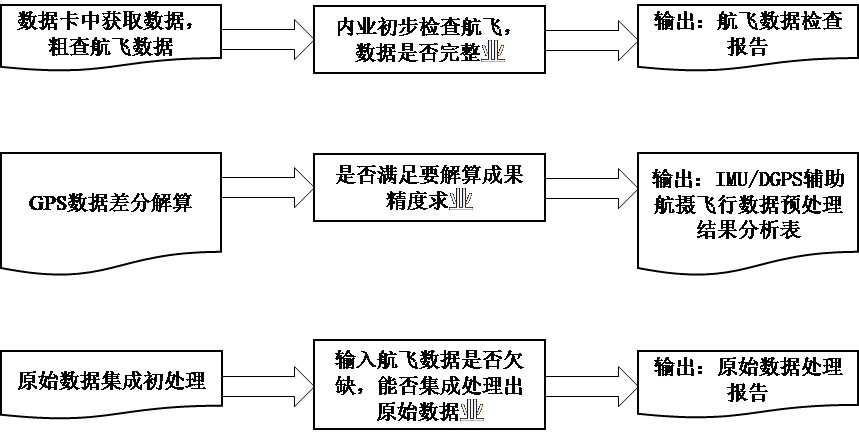
\includegraphics[width=0.8\textwidth]{images/chapter06/ch6_image62.png}
\caption{数据预处理的质量控制流程图}\label{fig:data-preprocess-qc}
\end{figure}

\paragraph{6.4.3.2 ContextCapture平台}\label{contextcaptureux5e73ux53f0}

ContextCapture实景三维建模软件，前身是较为知名的Smart3D Capture。Context Capture软件支持多种数据格式，是目前较为常用的倾斜影像数据处理软件，成果可在多种平台上浏览。该软件可以实现集群运算，多台计算机为同一测区工程作业。Context Capture主要包括：Center Master、Settings、Center Engine、Viewer。

Master负责创建工程、查看任务进度。Settings负责为Engine设置路径。Engine是引擎端，提交空三和重建任务后，可开启引擎进行计算。Viewer加载三维模型进行浏览和量测。

ContextCapture软件具有高性能、品质稳健、兼容性好、可扩展、可移植性强等特点。支持多种数据源，兼容各种航摄相机系统（Pictometry、Midas、AMC、A3等），能输出OBJ、OSGB、DAE、XML等通用兼容格式，能方便地导入各种主流GIS平台及三维编辑软件。

\subsection{BIM模型在水利工程中的作用与融合}

如果说倾斜摄影强调 ``真实还原现场''，那么BIM则强调 ``精细表达工程构件''。在水利工程中，BIM模型可对坝体分缝、闸门结构、启闭机、泵房机组、廊道、管线和附属建筑等对象进行分层组织，并记录构件编码、材质、尺寸、设备参数和运维属性。这种语义化能力使BIM模型非常适合支撑工程设计管理、运维台账和构件级查询。

\textbf{IFC标准在水利BIM中的应用}：BIM数据交换通常采用IFC（Industry Foundation Classes）标准，这是一种行业中立的开放格式，支持跨多个应用平台的数据互操作。在水利工程中，常用IFC 4.0版本定义坝体构件、闸门、泵房等对象。例如，一个混凝土重力坝可分解为多个IFCStructuralMember对象（代表分缝单元），每个单元记录其位置、尺寸和材料参数；闸门则用IfcDoor及其性质集（IfcPropertySet）来表示开度、操作机制等运维属性。IFC的优点是数据完整性高、支持模型版本管理，但缺点是文件体积通常较大（几百MB到几GB），不适合直接在Web浏览器中加载。

\textbf{BIM模型轻量化转换流程}：为解决IFC在网络传输和实时渲染中的性能瓶颈，通常需将IFC模型转换为轻量化格式。常见的转换流程为：（1）IFC导入CAD或BIM编辑软件（如Revit、Civil 3D、BricsCAD）；（2）进行模型简化和优化，包括删除冗余面片、合并相邻构件、简化复杂管线；（3）导出为中间格式如obj、gltf或专有格式；（4）进一步优化为3D Tiles或glTF 2.0 KHR\_draco\_mesh\_compression格式，实现几何压缩；（5）上传至Web服务器，通过CDN分发。这一流程可将模型体积压缩至原始IFC的1-5\%，保留足够的几何精度（通常为厘米级）。

\textbf{语义信息保留策略}：在轻量化过程中，构件的语义信息（如材料、位置、设备参数）必须保留。采用的策略是：（1）将IFC中的属性集转换为glTF扩展中的自定义JSON元数据，存储在每个模型节点（mesh）中；（2）建立构件ID与数据库表的映射，当用户点击模型上的构件时，通过ID查询实时监测数据、运维历史等；（3）对重要构件（如大坝表孔闸门）单独维护高精度BIM模型，其他次要构件则采用简化模型。这样可确保既有渲染性能，又不丢失工程管理所需的信息。

在智慧水利平台中，BIM与倾斜摄影的融合通常遵循 ``统一坐标基准、保留语义信息、按场景分层加载'' 的原则。对于核心建筑物内部结构和机电设备，可优先使用BIM模型表达；对于库区地形、岸坡、周边建筑与道路环境，可优先使用倾斜摄影模型表达；对于两者交界区域，则通过坐标校准、模型裁剪和图层切换等方式实现统一展示。这样既能保证整体场景的真实性，也能保留工程构件的可管理性。

\subsection{工程三维模型构建流程}

为了提高建模效率，大坝数字化建模可以采用工作站并行 GPU 框架架构和专用硬盘存储数据，保证数据快速读取及高效计算。除此以外，为了保证建模精度和效果，还要选择一款性能强大的建模软件，倾斜摄影三维建模软件众多，如Bentley公司的ContextCapture、Skyline公司的PhotoMesh、Astrium公司的街景工厂等。

以采用ContextCapture作为建模软件为例，介绍建模流程。ContextCapture三维建模是利用空中三角测量算法，空中三角加密提取5个视角的影像特征点，将特征点与同名点进行匹配，通过反向结算确定影像之间的相对关系。特征点选取主要原则为：

（1）特征点应选刺在航向及旁向六片（或五片）重叠范围内，使布设的特征点能尽量公用。

（2）特征点尽量布设在旁向重叠的中线附近。旁向重叠过小，相邻航线像控点不能公用时，应分别布点。当旁向重叠过大使相邻航线的点不能公用时，亦应分别布点。

（3）当特征点为平高点时，实地选点时选择影像清晰的明显地物点，如接近线状地物的交点，地物拐角点等实地辨认误差小于图上0.1mm的地物点，当像控点为高程点时，要优选局部高程变化不大的地物目标点，不可在弧形地物及高程变化较大的斜坡处选刺像控点。

ContextCapture通过空中三角加密计算出大量的连接点，利用这些连接点构建不规则三角网TIN，生成三维模型的基本框架，将三维模型白模和表面的纹理信息进行自动映射，从而获取具有真实、自然纹理的高分辨率实景三维模型。

ContextCapture整个建模过程如下：

（1）新建工程

双击打开Context Capture Center Master，点击New project，会生成相应的文件夹，以及文件后缀为ccm的文件。

（2）导入数据

导入倾斜影像数据，并导入相应五视镜头的相机参数以及POS数据。

（3）空三加密

导入数据之后，在surveys界面下标记少许几个像控点的位置，即刺点工作，完成后提交空三任务。经过首次空三计算之后，可以使像控点与影像大致关联，方便作业人员继续完成控制点刺点工作。一般在标记两到三张影像之后，会更加精确的关联到其他影像。在影像上刺点时，要根据现场照片以及结合影像中周围地物仔细确认像控点位置，避免刺点错误，否则可能会导致空三结果质量变差甚至导致空三任务失败。为提高空三任务的精度，刺点作业时要尽可能的多的标记像控点相关联的影像。一般情况下，倾斜视角影像中像控点标志的变形较大，可能无法判断正确的点位。垂直影像变形较小，先从下视开始刺点，之前已编辑过影像名称，就可以快速的定位到下视影像进行作业。刺点作业结束后，在3D view 下查看像控点的状态，确保所有像控点均已进行影像刺点，提交空三任务并打开引擎调动其他计算机开始作业。

（4）用户连接点优化方案

空三任务结束后，空三成果质量除了查看空三质量报告外，3D view下的密集匹配点云的状态也是重要的参考。在部分场景纹理偏弱，计算机不能识别，匹配难度增加时，就会出现部分升起以及下降的影像，这些影像没有参与计算或计算结果存在着错误，同样，这些区域的密集匹配点云也存在着错误。在Photos面板下可以查看这些影像具体拍摄的场景。若对这些影像不进行处理，则重建的三维模型在此部分由于三角网的连接错误，即使进行纹理映射后，模型也会出现升起或者下降的部分，不仅不符合现实世界，三维模型的精度也无法得到保证。

针对上述情况，通过添加用户连接点进行调节。采用人机交互的方式，人工判读标记明显的地物特征，引导计算机去识别，使这些影像重新参与计算，恢复其正确的姿态和位置。用户连接点的添加过程如下：

选中升起或下降的影像，用户连接点的添加在Surveys面板下进行。在影像中挑选标志性的地物，该地物应具备明显、稳固，不易移动的特征。经多次实验发现，升起以及下降的影像通常是一个方向的，若用户连接点刺点仅在该方向影像上进行，则添加用户连接点无效。需要对多个方向影像进行刺点，方便联合计算恢复问题影像的正确姿态和位置。由于对影像文件名称已经进行编辑，五视方向容易找到。每个方向需刺点的影像数约为五张，用户连接点的个数不需要过多，均匀分布在升起以及下降的区域中。用户连接点添加结束后，重新提交空三任务。由于人工辅助计算机确定难以匹配的位置，经过空三重新计算后，这些升起以及下降的影像可以恢复其正确的位置和姿态。查看密集匹配点云结果，结果趋于平整，没有升起以及下降的部分。以此方案添加连接点，可以改善空三成果的质量并减少提交空三任务的次数，节约整体建模时间。

（5）三维重建

空三任务完成，满足建模条件后，建立新的三维重建任务，设置参数，选择坐标系，此时默认建模区域是一个整块，软件会给出预计最大内存使用值，需要结合自身计算机内存情况，对建模区域进行划分，一般选取Regular planar grid 进行划分，设定瓦片大小的值，确定划分的瓦片个数。参数设置好之后，提交新的生产，选择产品形式为3D mesh。

产品格式一般设置为Open Scene Graph binary (OSGB)格式，选择目标坐标系统，定义生产模型范围，最后选择模型输出位置。

\subsection{BIM与GIS融合技术}

\textbf{CityGML与IFC的映射关系}：在智慧水利的数字孪生场景中，需要同时处理两种语义模型：IFC侧重于工程构件的设计和运维属性，CityGML则是地理信息领域的标准3D城市模型格式。两者的映射关系如下：IFC中的IfcBuildingStorey对应CityGML中的CityObjectGroup（可代表一个建筑楼层或功能区）；IFC中的IfcSpace对应CityGML的Room；IFC中的构件材料属性可映射到CityGML的Appearance模块。通过建立映射规则库，可实现IFC模型向CityGML的自动转换，使BIM模型能与GIS底图无缝融合。在实际应用中，可采用FME（Feature Manipulation Engine）或自定义转换脚本完成转换，保留关键属性同时简化数据结构。

\textbf{3D Tiles规范在BIM集成中的作用}：3D Tiles是Cesium开发的轻量级3D地理空间数据规范，采用分级存储和流式传输机制，特别适合海量BIM模型的Web发布。3D Tiles支持多种几何类型（包括glTF 2.0、instanced 3D models等）和LOD机制，可根据网络带宽和设备性能动态加载不同细节级别的模型。对于BIM模型，转换为3D Tiles的流程为：（1）将IFC或glTF转换为Tileset JSON结构；（2）为每个构件定义包围盒和几何边界；（3）配置特征表（Feature Table）存储构件ID、属性等元数据；（4）按四叉树或八叉树组织瓦片，支持并行加载。这种方式可将数GB的BIM模型压缩至几百MB，并通过CDN加速分发。

\textbf{水库大坝BIM模型在三维平台上的加载与交互}：以某大型水库的BIM场景为例，展示BIM与GIS融合的具体实现。该场景包含一座混凝土重力坝（坝高140米，坝长1200米）及其配套工程。

\textbf{模型构成}：大坝本体分为258个分缝单元，每个单元独立为IFC中的StructuralMember对象；溢洪道、泄洪洞、发电站分别为独立的IfcBuilding；廊道、管线等辅助设施记录在IfcFurniture和IfcFlowSegment中。

\textbf{模型转换与优化}：原始IFC文件约2.8GB，通过以下步骤转换为3D Tiles：
\begin{enumerate}
\item 在Revit中按功能模块分解模型（坝体、溢洪道、发电站等），每个模块导出独立的glTF文件；
\item 使用glTF-Pipeline进行压缩（启用draco网格压缩，精度设为0.01米）；
\item 使用3D Tiles Tools将各模块转换为.3dtiles格式，总体积降至320MB；
\item 按距离设置LOD：距离>2km加载LOD0（仅坝体简化模型），距离1-2km加载LOD1（坝体+主要附属建筑），距离<1km加载LOD2（全部细节）。
\end{enumerate}

\textbf{交互功能实现}：当用户在Cesium三维场景中点击大坝上的某个分缝单元时，触发拾取事件，获取该单元的ID后查询数据库，展示其关联的监测数据（如该分缝的沉降、裂缝宽度、渗压等）。在右侧面板显示该构件的属性信息（如位置、混凝土标号、施工时间等），用户可进一步点击跳转至该单元的历史监测曲线或维护工作单。如果该分缝监测数据超过警戒值，对应的模型面片会高亮显示（如变为红色）并闪烁提醒。

这一集成方案既充分利用了BIM的语义完整性，也借助GIS的空间可视化优势，为运维人员提供了直观的工程状态感知和快速的信息查询入口。

\subsection{模型成果分析}

\paragraph{6.4.5.1 模型复杂度分析}\label{ux6a21ux578bux590dux6742ux5ea6ux5206ux6790}

模型成果格式主要为OSGB格式以及S3C格式，OSGB格式模型与相对应的OBJ格式模型导入第三方平台进行模型修饰。S3C文件是分块模型的索引，可以全场景加载三维模型。将S3C格式的成果文件加载到Viewer模型浏览平台上，通过旋转浏览可以看出重建区域的三维实景模型中地物相对位置的正确与否。根据《三维地理信息模型数据产品规范》所规定，可以进一步评价模型达到的构建级别要求。

\paragraph{6.4.5.2 模型几何精度分析}\label{ux6a21ux578bux51e0ux4f55ux7cbeux5ea6ux5206ux6790}

为验证倾斜摄影测量技术生产的三维模型精度能否满足一些测绘应用如立面测绘、大比例尺地形图绘制、地籍测量等等，需要对模型几何精度进行分析。Context Capture生产的三维模型，加载到Viewer浏览平台上可以进行三维坐标量测、距离量测、高差计算及其他分析功能。在测区内选取20个显著特征点，选点时要在现场和模型中可以清晰找到，利用RTK 进行实测其三维坐标并将其作为真值，通过模型浏览平台采集相对应位置三维坐标，计算两者之间差值并进行统计。按照如下中误差公式可以计算面中误差及高程中误差，并进行模型几何精度评定。

${m_x} = \sqrt{\frac{1}{n}\sum\limits_{i = 1}^n {{{\left( {D{X_i}} \right)}^2}} } $ (6.4.1)

${m_x} = \sqrt{\frac{1}{n}\sum\limits_{i = 1}^n {{{\left( {D{X_i}} \right)}^2}} } $(6.4.2)

${m_x} = \sqrt{\frac{1}{n}\sum\limits_{i = 1}^n {{{\left( {D{X_i}} \right)}^2}} } $(6.4.3)

通过计算构建的三维模型点位中误差、平面最小误差、最大误差值、高程中误差、高程最小误差、最大误差值，根据《三维地理信息模型数据产品规范》规定，即可评价模型满足的等级要求。

\paragraph*{小结}

本节说明了BIM模型和倾斜摄影模型在智慧水利三维场景中的分工与融合方式。前者强调工程语义与构件管理，后者强调空间真实感与环境还原，两者与GIS空间底座结合后，才能为后续的数字孪生平台提供可靠的模型基础和统一的场景表达能力。

\section{水利工程数字孪生架构}

数字孪生并不是孤立增加的一层可视化功能，而是建立在GIS空间底座、BIM工程语义、倾斜摄影实景模型和实时监测数据之上的综合应用架构。只有当前述模型、图层和业务数据可以统一组织并持续更新时，数字孪生平台才能真正支撑工程态势感知、预警分析与辅助决策。

\paragraph*{数字孪生概述}

数字孪生（Digital Twin）是充分利用物理模型、传感器更新、运行历史等数据，集成多学科、多物理量、多尺度、多概率的仿真过程，在虚拟空间中完成映射，从而反映相对应的实体装备的全生命周期过程\cite{glaessgen2012}。在智慧水利领域，数字孪生技术通过构建水利设施的高保真数字模型，实现物理水利工程与数字模型的实时同步和交互。

\paragraph{数字孪生的核心特征}\label{ux6570ux5b57ux5b6aux751fux7684ux6838ux5fc3ux7279ux5f81}

\textbf{1. 高保真度建模} - 几何保真：精确再现水利设施的几何形状和空间关系 - 物理保真：准确模拟水力学、结构力学等物理过程 - 行为保真：真实反映系统的动态响应和运行规律

\textbf{2. 实时数据同步} - 双向数据流：物理实体向数字模型传输状态数据，数字模型向物理实体反馈控制指令 - 多源数据融合：整合监测传感器、遥感影像、业务系统等多源数据 - 低延迟更新：确保数字模型能够实时反映物理实体的最新状态

\textbf{3. 预测性分析} - 状态预测：基于历史数据和当前状态预测未来发展趋势 - 故障诊断：通过模式识别和异常检测提前发现潜在问题 - 优化决策：利用仿真分析优化运行参数和维护策略

\subsection{数字孪生五维模型与技术架构}

\paragraph{数字孪生五维模型}\label{ux6570ux5b57ux5b6aux751fux4e94ux7ef4ux6a21ux578b}

根据数字孪生理论，水利工程数字孪生包含五个维度：

\textbf{1. 物理实体（Physical Entity）} - 水利基础设施：大坝、闸站、渠道、管网等 - 水文要素：河流、湖泊、地下水、降雨等 - 设备装置：监测仪器、控制设备、机电设备等

\textbf{2. 数字模型（Digital Model）} - 几何模型：三维CAD模型、BIM模型、点云模型 - 物理模型：水动力学模型、结构力学模型、热力学模型 - 数据模型：监测数据、历史数据、预测数据

\textbf{3. 数据连接（Data Connection）} - 传感器网络：IoT传感器、自动监测站、遥感卫星 - 通信网络：5G/4G、光纤、卫星通信、工业以太网 - 数据接口：API接口、数据库接口、文件传输协议

\textbf{4. 服务应用（Service）} - 监测服务：实时监测、状态展示、趋势分析 - 仿真服务：洪水演进、结构分析、调度优化 - 预警服务：异常检测、风险评估、应急响应

\textbf{5. 数据处理（Data Processing）} - 数据清洗：异常值检测、缺失值补充、噪声过滤 - 数据融合：多源数据整合、时空配准、不确定性处理 - 智能分析：机器学习、深度学习、知识推理

\paragraph{技术架构设计}\label{ux6280ux672fux67b6ux6784ux8bbeux8ba1}

\begin{lstlisting}[language=Python]
class WaterDigitalTwin:
    """水利工程数字孪生系统"""
    
    def __init__(self, project_config):
        self.project_id = project_config['project_id']
        self.physical_entity = PhysicalEntity(project_config)
        self.digital_model = DigitalModel(project_config)
        self.data_connector = DataConnector(project_config)
        self.service_layer = ServiceLayer(project_config)
        self.data_processor = DataProcessor(project_config)
        
    def initialize_twin(self):
        """初始化数字孪生系统"""

        self.digital_model.build_geometric_model()
        self.digital_model.build_physical_model()
        self.digital_model.build_data_model()

        self.data_connector.establish_sensor_connections()
        self.data_connector.setup_communication_protocols()

        self.service_layer.start_monitoring_service()
        self.service_layer.start_simulation_service()
        self.service_layer.start_analysis_service()

        self.data_processor.setup_data_pipelines()
        
    def sync_with_physical(self):
        """与物理实体同步"""

        sensor_data = self.data_connector.collect_sensor_data()

        processed_data = self.data_processor.process_real_time_data(sensor_data)

        self.digital_model.update_model_state(processed_data)

        simulation_results = self.digital_model.run_simulation()

        control_commands = self.service_layer.generate_control_commands(simulation_results)
        
        return {
            'model_state': self.digital_model.get_current_state(),
            'simulation_results': simulation_results,
            'control_commands': control_commands
        }
        
    def predict_future_state(self, time_horizon):
        """预测未来状态"""
        current_state = self.digital_model.get_current_state()
        historical_data = self.data_processor.get_historical_data()

        prediction_model = self.service_layer.get_prediction_model()
        future_states = prediction_model.predict(
            current_state, 
            historical_data, 
            time_horizon
        )
        
        return future_states
\end{lstlisting}
\subsection{典型应用案例}

\paragraph{大坝安全监测数字孪生}\label{ux5927ux575dux5b89ux5168ux76d1ux6d4bux6570ux5b57ux5b6aux751f}

以某重力坝为例，构建大坝安全监测数字孪生系统：

\textbf{物理实体组成}： - 大坝本体：混凝土重力坝，坝高185m，坝顶长度2309m - 监测设备：变形监测点412个，渗压监测点156个，应力应变监测点89个 - 环境要素：库水位、温度、地震、降雨等

\textbf{数字模型构建}：

\begin{enumerate}
\def\labelenumi{\arabic{enumi}.}
\tightlist
\item
  \textbf{几何模型}：基于BIM技术构建精细化三维模型
\item
  \textbf{有限元模型}：建立结构分析有限元模型
\item
  \textbf{渗流模型}：构建三维渗流分析模型
\item
  \textbf{温度场模型}：建立温度场分析模型
\end{enumerate}

\textbf{核心功能实现}：

\begin{lstlisting}[language=Python]
class DamDigitalTwin(WaterDigitalTwin):
    """大坝数字孪生系统"""
    
    def __init__(self, dam_config):
        super().__init__(dam_config)
        self.dam_model = DamStructuralModel(dam_config)
        self.seepage_model = SeepageModel(dam_config)
        self.temperature_model = TemperatureModel(dam_config)
        
    def analyze_dam_safety(self):
        """大坝安全分析"""

        displacement_data = self.get_displacement_monitoring_data()
        seepage_data = self.get_seepage_monitoring_data()
        stress_data = self.get_stress_monitoring_data()

        structural_response = self.dam_model.analyze_structural_response(
            displacement_data, stress_data
        )

        seepage_state = self.seepage_model.analyze_seepage_condition(
            seepage_data
        )

        thermal_effect = self.temperature_model.analyze_thermal_effect()

        safety_assessment = self.evaluate_dam_safety(
            structural_response, seepage_state, thermal_effect
        )
        
        return {
            'structural_analysis': structural_response,
            'seepage_analysis': seepage_state,
            'thermal_analysis': thermal_effect,
            'safety_level': safety_assessment['safety_level'],
            'risk_factors': safety_assessment['risk_factors'],
            'recommendations': safety_assessment['recommendations']
        }
        
    def predict_dam_behavior(self, forecast_period):
        """预测大坝行为"""

        historical_data = self.get_historical_monitoring_data()

        displacement_predictor = DisplacementPredictor()
        displacement_predictor.train(historical_data['displacement'])
        
        seepage_predictor = SeepagePredictor()
        seepage_predictor.train(historical_data['seepage'])

        future_displacement = displacement_predictor.predict(forecast_period)
        future_seepage = seepage_predictor.predict(forecast_period)

        numerical_results = self.dam_model.simulate_future_behavior(
            future_displacement, future_seepage, forecast_period
        )
        
        return {
            'predicted_displacement': future_displacement,
            'predicted_seepage': future_seepage,
            'numerical_simulation': numerical_results,
            'confidence_interval': self.calculate_prediction_confidence(),
            'alert_thresholds': self.get_safety_thresholds()
        }
\end{lstlisting}

\paragraph{智能调度数字孪生}\label{ux667aux80fdux8c03ux5ea6ux6570ux5b57ux5b6aux751f}

以流域水资源调度为例：

\textbf{系统架构}： - 物理流域：干支流水系、水库群、闸坝群、引调水工程 - 数字流域：水文模型、水力学模型、调度优化模型 - 智能决策：多目标优化、智能算法、决策支持

\textbf{关键技术}：

\begin{lstlisting}[language=Python]
class BasinDigitalTwin(WaterDigitalTwin):
    """流域数字孪生系统"""
    
    def __init__(self, basin_config):
        super().__init__(basin_config)
        self.hydrological_model = HydrologicalModel(basin_config)
        self.hydraulic_model = HydraulicModel(basin_config)
        self.optimization_model = OptimizationModel(basin_config)
        
    def real_time_dispatch(self):
        """实时调度决策"""

        water_levels = self.get_real_time_water_levels()
        inflows = self.get_real_time_inflows()
        weather_forecast = self.get_weather_forecast()

        flow_forecast = self.hydrological_model.forecast_flow(
            inflows, weather_forecast
        )

        hydraulic_state = self.hydraulic_model.calculate_hydraulic_state(
            water_levels, flow_forecast
        )

        optimal_strategy = self.optimization_model.optimize_dispatch(
            hydraulic_state, flow_forecast
        )

        risk_assessment = self.assess_dispatch_risk(optimal_strategy)
        
        return {
            'dispatch_strategy': optimal_strategy,
            'risk_level': risk_assessment['risk_level'],
            'alternative_strategies': optimal_strategy['alternatives'],
            'expected_benefits': optimal_strategy['benefits']
        }
\end{lstlisting}
\subsection{关键技术挑战与解决方案}

\paragraph{技术挑战}\label{ux6280ux672fux6311ux6218}

\textbf{1. 模型保真度与计算效率的平衡} - 高保真模型计算复杂度高，难以实现实时计算 - 简化模型精度不足，影响分析结果可靠性

\textbf{解决方案}： - 多分辨率建模：根据应用需求采用不同精度的模型 - 代理模型技术：使用机器学习构建高效代理模型 - 并行计算：利用GPU、集群等并行计算资源

\textbf{2. 多源数据融合与不确定性处理} - 数据来源多样，格式标准不统一 - 数据质量参差不齐，存在缺失、噪声、异常 - 不确定性传播影响分析结果可信度

\textbf{解决方案}： - 数据标准化：建立统一的数据标准和接口规范 - 数据质量控制：实施多层次的数据质量检查和清洗 - 不确定性量化：采用概率方法量化和传播不确定性

\textbf{3. 实时性与准确性的协调} - 实时应用要求快速响应，限制了分析深度 - 准确分析需要时间，影响决策时效性

\textbf{解决方案}： - 分层计算架构：快速响应层+深度分析层 - 预计算策略：预先计算常见场景的分析结果 - 增量更新：仅对变化部分进行重新计算

\subsection{发展趋势与展望}

\paragraph{技术发展趋势}\label{ux6280ux672fux53d1ux5c55ux8d8bux52bf}

\textbf{1. 人工智能深度融合} - 深度学习支撑模型构建和参数识别 - 强化学习优化控制策略 - 知识图谱增强领域知识表达

\textbf{2. 边缘计算与云边协同} - 边缘侧实现低延迟响应 - 云端提供强大计算能力 - 云边协同优化资源配置

\textbf{3. 元宇宙技术融合} - 虚实融合的沉浸式体验 - 多人协同的虚拟工作空间 - 区块链保障数据可信

\textbf{4. 自主进化能力} - 自适应模型参数调整 - 自主学习优化算法 - 自我诊断修复能力

\paragraph{应用前景展望}\label{ux5e94ux7528ux524dux666fux5c55ux671b}

\textbf{1. 全生命周期管理} - 从规划设计到运行维护的全过程数字化 - 基于数字孪生的工程全生命周期优化 - 历史数据积累驱动的知识传承

\textbf{2. 跨流域协同调度} - 多流域数字孪生系统互联互通 - 区域水资源统一调度优化 - 极端事件下的应急协调响应

\textbf{3. 智慧城市水务} - 城市水循环数字孪生 - 智能供排水系统 - 海绵城市运行优化

\textbf{4. 生态环境保护} - 河湖生态系统数字孪生 - 水生态修复效果预测 - 生态调度决策支持

\paragraph*{小结}

数字孪生技术为智慧水利发展注入了新的活力，通过构建高保真的数字模型，实现了物理水利工程与数字世界的深度融合。本节详细介绍了数字孪生的基本概念、技术架构、应用案例和发展趋势，为读者提供了全面的技术视角。

数字孪生技术的成功应用需要多学科知识的深度融合，包括水利工程、计算机科学、数据科学、人工智能等。随着技术的不断进步和应用实践的深入，数字孪生必将成为智慧水利建设的重要技术支撑。

\section*{本章小结}

本章系统介绍了三维可视化、GIS地图服务、BIM建模和数字孪生在智慧水利中的关键技术与应用。WebGL和Three.js为Web端3D交互式展示奠定了基础，无需专业图形软件即可在浏览器中呈现复杂的水利工程场景。地形、水体、建筑、植被等多类地物的精细建模，需要综合运用LiDAR点云、倾斜摄影、无人机遥感等多源数据采集与处理技术。

GIS地图服务（Cesium、Leaflet等）将大尺度区域空间数据与实时监测数据进行融合，支撑了水资源管理、防洪预警、生态监测等应用。BIM模型的建立与维护贯穿工程规划、设计、施工、运维全生命周期，提供了协同管理平台。数字孪生通过构建物理工程的数字镜像，实现了实时感知、动态模拟、优化决策的闭环，是水利工程向智能化升级的核心技术。

本章通过大坝安全监测、河道防洪决策、流域水资源调度等典型应用案例，展示了如何综合运用这些技术解决复杂的水利工程问题。随着AI、边缘计算、元宇宙等新技术的持续演进，数字孪生将为水利行业的数字化转型和智能化升级提供强大支撑。

\section*{小结}

本章从三维图形学基础、WebGL与Three.js开发框架、GIS地图服务集成、BIM与倾斜摄影建模，到数字孪生架构设计，系统介绍了智慧水利平台三维场景技术的基础知识体系。三维渲染管线、场景组织、坐标变换和渲染优化是理解三维可视化的基础；GIS服务和BIM模型为水利场景提供了空间底座和工程语义；数字孪生则将物理工程、数字模型、实时数据和智能服务统一起来。本章内容为第7章的数据可视化展示提供了技术基础。

\section*{章末交付物}

完成本章学习后，建议提交一张“三维场景数据流程图”或等价说明文档，至少包括：

\begin{itemize}
\item 原始空间数据来源，如地形、影像、BIM模型和监测点位；
\item 模型加工、坐标统一、轻量化与切片发布流程；
\item 前端加载方式和业务数据叠加方式；
\item 性能优化策略，如LOD、缓存和按需加载。
\end{itemize}

\section*{思考题与练习题}

\begin{enumerate}

\item[\textbf{概念理解题}]

\item 分析三维可视化技术在智慧水利中的应用价值，说明WebGL和Three.js各自的特点和适用场景。

\item 论述三维建模中地形、水体、建筑和植被建模的关键技术，说明各类模型的数据来源和处理方法。

\item 比较点云、体素、网格等三维数据结构的特点，分析在不同水利应用场景中的选择依据。

\item 解释GIS地图服务（Cesium、Leaflet）在实现大尺度区域监测和空间决策支持中的核心功能和优势。

\item 论述BIM模型在水利工程全生命周期中的应用，说明BIM与三维场景、GIS系统的数据集成方式。

\item 分析数字孪生技术中物理工程与数字系统的映射机制，说明实时同步、模型更新的关键技术。

\item 论述大数据、AI、云边协同等新技术对数字孪生系统的支撑作用，展望智慧水利的发展前景。

\item 比较传统水利工程管理与基于数字孪生的智能管理方式的差异，分析数字孪生带来的管理模式创新。

\item[\textbf{设计与编程题}]

\item 使用Three.js开发一个水库三维场景，包含坝体、库区水面、周边地形，支持旋转、缩放、漫游等交互操作。

\item 基于Cesium框架，构建一个流域尺度的GIS监测平台，展示多个监测站的位置、实时数据和告警状态，支持点击查看详情。

\item 利用倾斜摄影数据和三维建模软件，为一个实际水利工程（如水闸、泵站）建立精细化BIM模型，实现与GIS系统的配准集成。

\item 设计一个大坝安全监测的数字孪生系统，将渗压、位移、应力等多物理场进行耦合模拟，实现实时风险评估和预警。

\item 开发一个流域水资源调度数字孪生，集成水文模型、水力学模型和优化决策模型，支持多目标调度方案的对比分析。

\item 构建一个水库应急管理数字孪生场景，将超标洪水等极端工况进行高保真模拟，为应急决策和预案制定提供支撑。

\item[\textbf{应用创新题}]

\item 设计一个基于数字孪生的防洪决策支持系统，说明如何将降雨预报、水位预报、流量预测等信息进行实时融合，支持防洪调度。

\item 提出一个跨流域水资源协调管理方案，利用数字孪生技术实现多个工程的协同运行，优化整体社会经济效益。

\end{enumerate}
